

\subsection{PDSurvey Platform}

	The public display survey (\textit{PDSurvey}) platform aims to facilitate the execution and evaluation of surveys on and for public displays. 
	The interactive survey platform, which can be embedded directly onto public displays and be used as a direct feedback channel from inside another application, can be split into three main parts: PDAdmin, PDServer, and PDClient (see figure \ref{fig:4-pdsurvey-platform}). \textit{PDAdmin} contains the administrative interface, allowing display providers to configure questionnaires for their public displays. \textit{PDServer} accommodates the REST service, the persistence layer, and the majority of the application logic. \textit{PDClient} is a web-based interface, containing one possibility for responding to the deployed surveys. 
	The code base of all three parts is deliberately separated from each other, allowing the independent refinement and less dependence between the frontend, the backend, and the server.

	\begin{figure}[btph]
	    \begin{center}
	        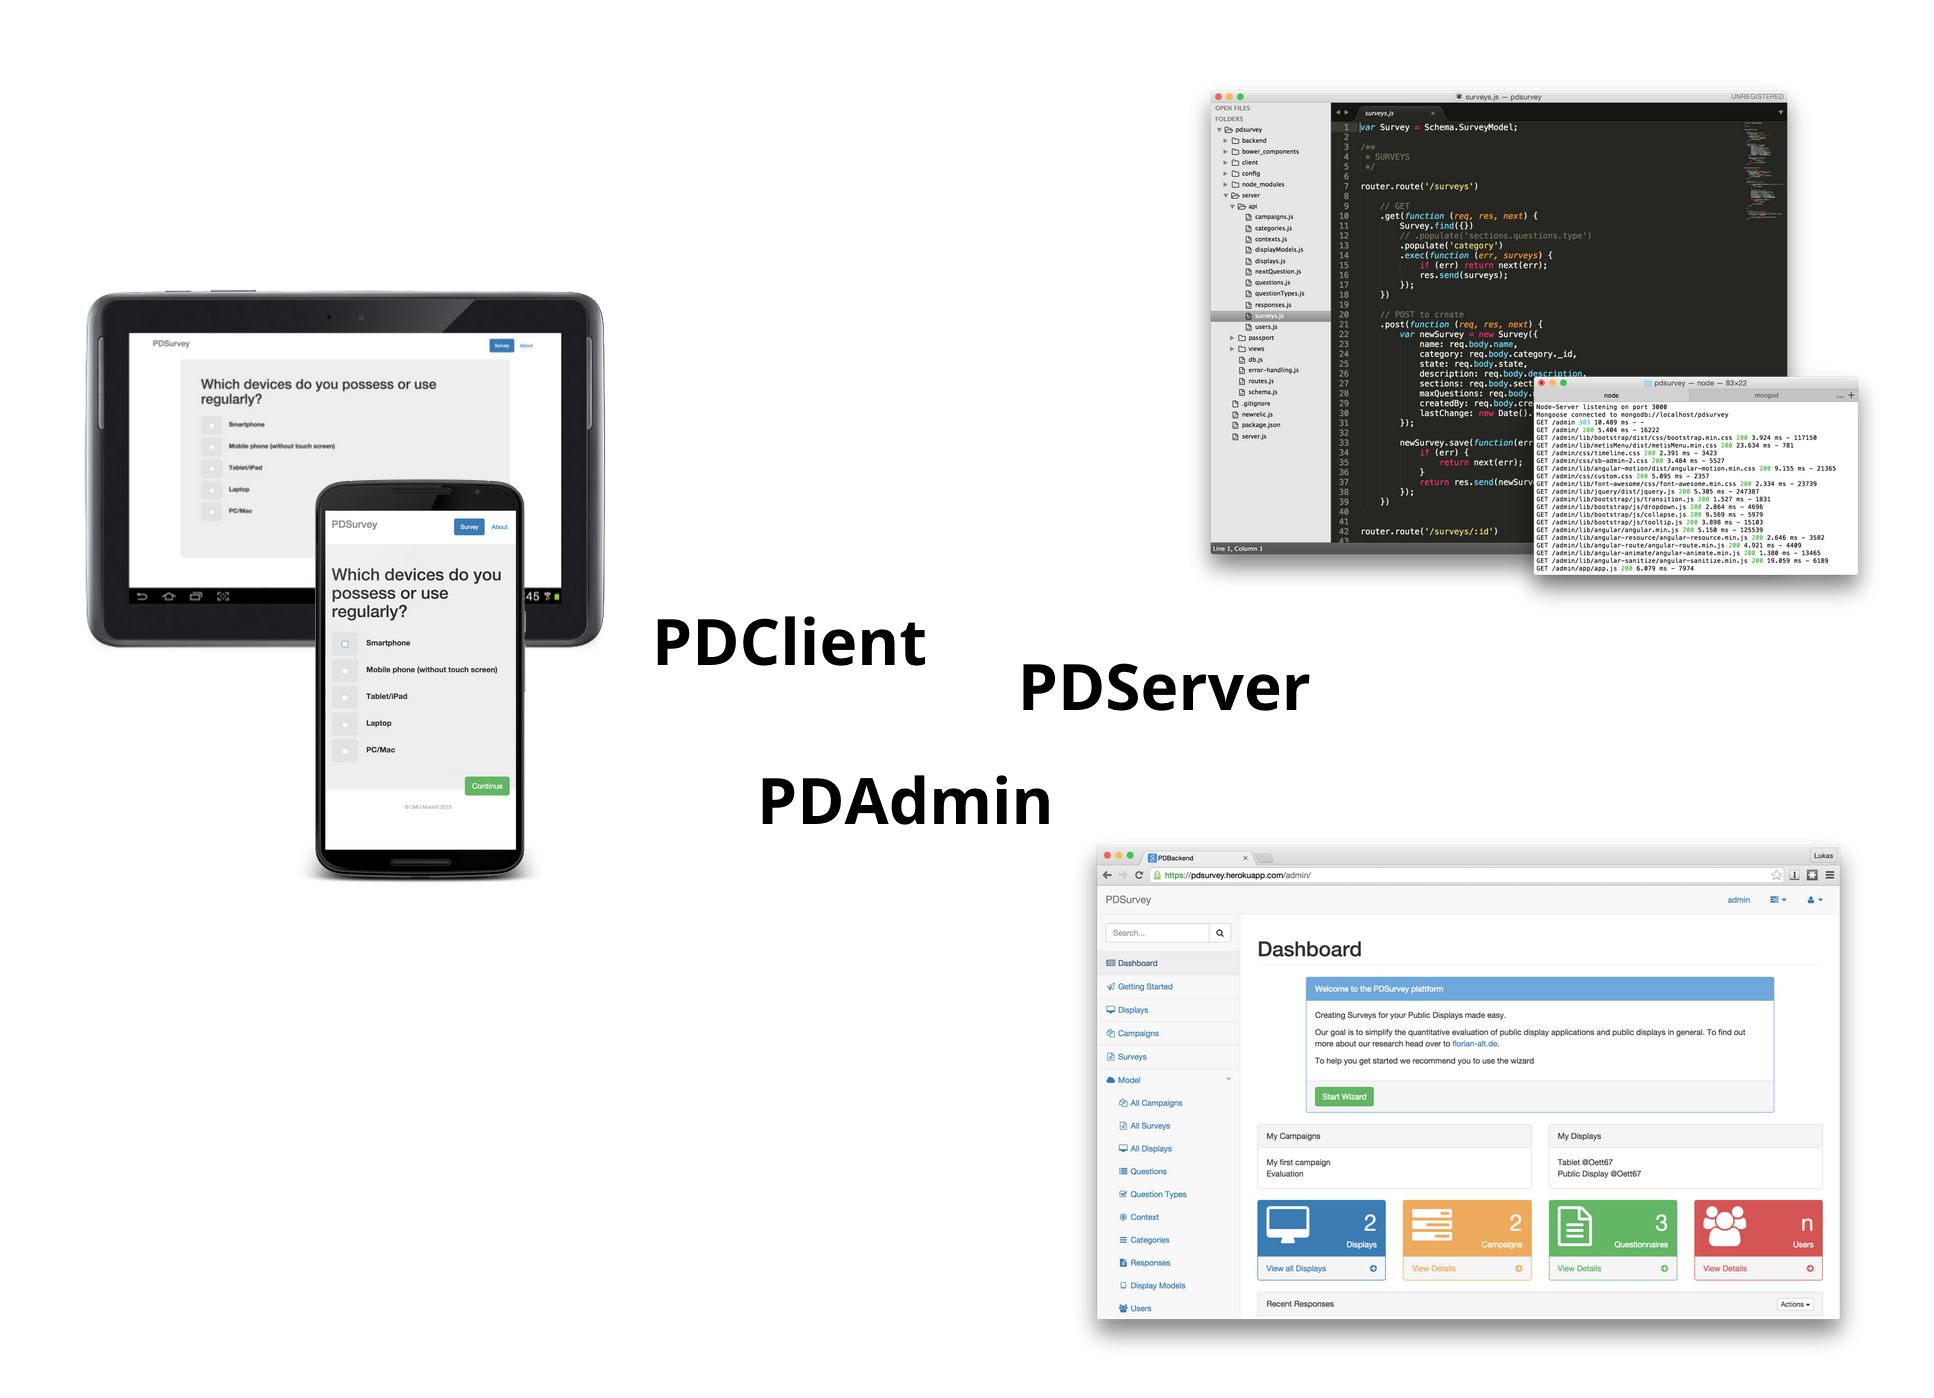
\includegraphics[width=.8\columnwidth]{img/screenshots/pdsurvey-overview/pdsurvey-platform.png}
	    \end{center}
	 \caption[Overview of the \textit{PDSurvey} platform]{Overview of the PDSurvey platform: (a) PDClient contains the responsive interface for PDs, (b) PDBackend is the entry point for administrators, (c) PDServer consists of Node.js and provides a REST API. }
	 \label{fig:4-pdsurvey-platform}
	\end{figure}



	\subsubsection{PDAdmin}

		For administrative purposes an admin interface was created, enabling display providers to create, manage and distribute surveys to public displays. Display providers have the ability to create their own questionnaires or to select from a list of standardized questionnaires (chapter \ref{chapter:literature-review}).
		The entry point for PDAdmin is the dashboard (see figure \ref{fig:pdadmin-dashobard}). There users get an overview of all relevant information such as how their campaigns are running, and how many responses have been submitted already. 
		% Wizard
		For new users, who haven't created any campaigns, questionnaires or displays yet, the \textit{Wizard} (see figure \ref{fig:pdadmin-wizard}) will be the best place to get started with the survey platform. Users get guided through the creation process of campaigns step by step.
		% Experts
		For more experienced users the navigation options \textit{Displays}, \textit{Campaigns}, and \textit{Surveys} are more advisable. 
		% Admins
		Administrators of the survey platform additionally have the ability to add new \textit{Users}, \textit{Question Types}, or research \textit{Categories}.


	% \begin{figure}%[btph]
	%     \begin{center}
	%         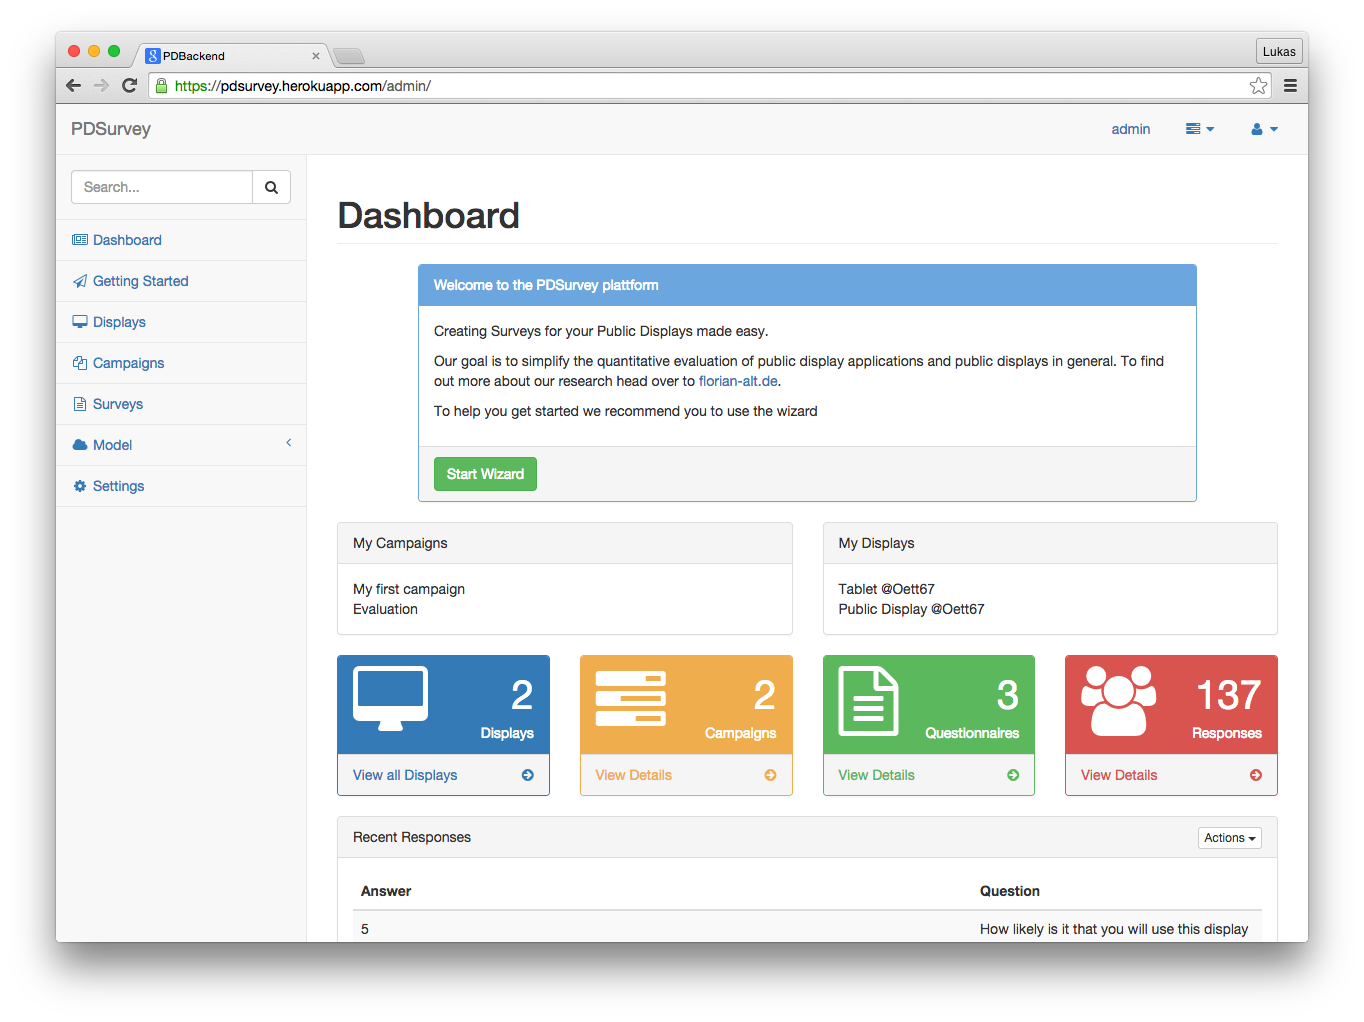
\includegraphics[width=.8\columnwidth]{img/screenshots/pdadmin/dashboard.png}
	%     \end{center}
	%  \caption[PDAdmin Dashboard]{Dashboard for PDAdmin}
	%  \label{fig:pdadmin-dashobard}
	% \end{figure}

	% \begin{figure}%[btph]
	%     \begin{center}
	%         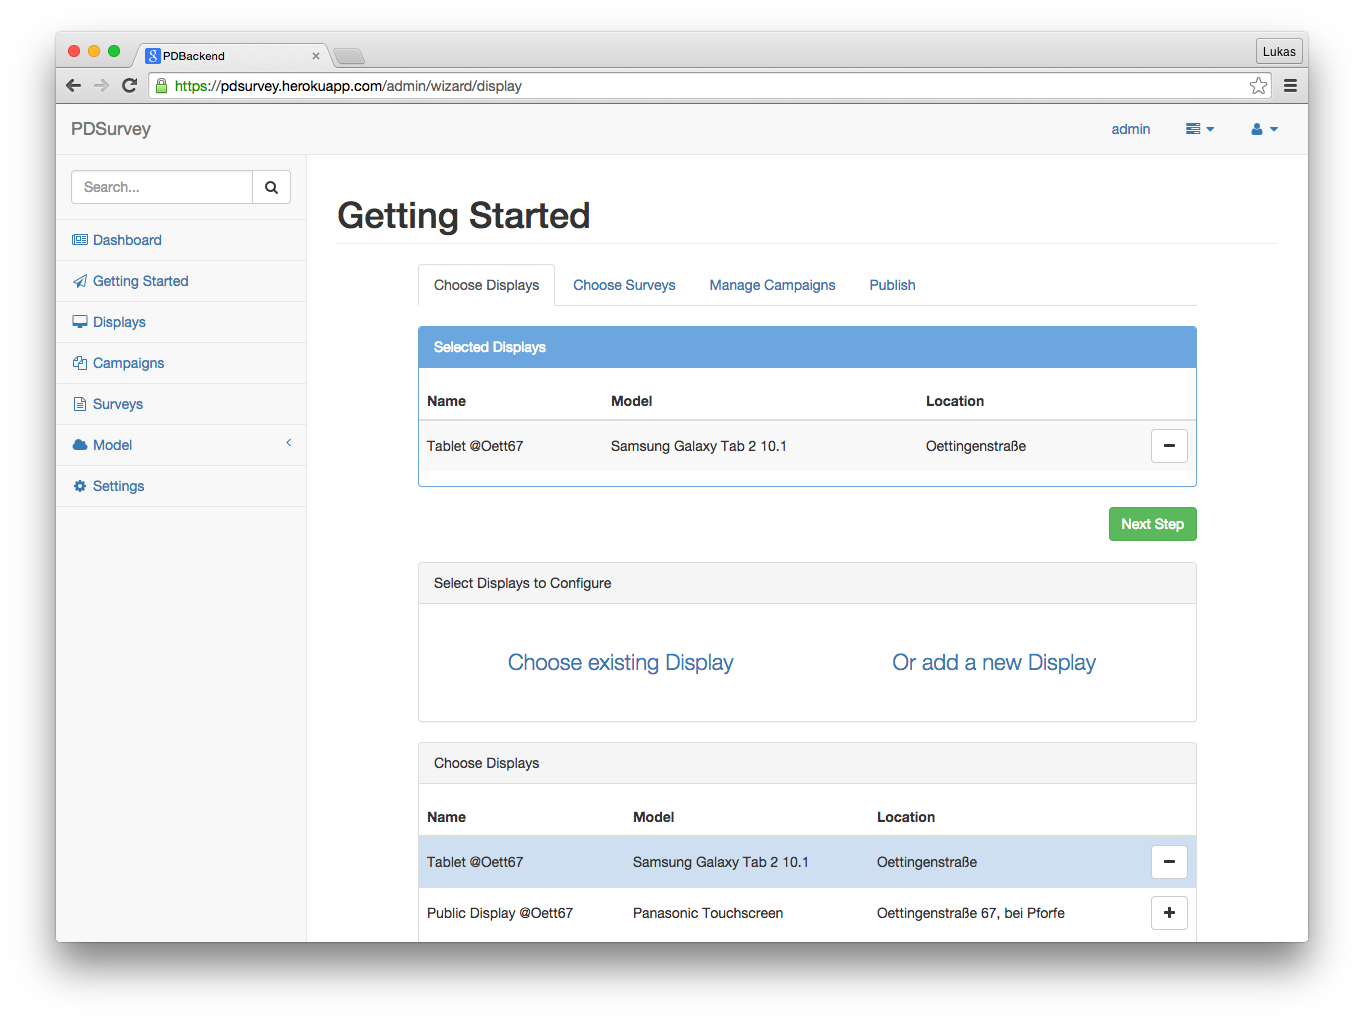
\includegraphics[width=.8\columnwidth]{img/screenshots/pdadmin/wizard-display_selected.png}
	%     \end{center}
	%  \caption[PDAdmin Wizard]{Wizard for PDAdmin}
	%  \label{fig:pdadmin-wizard}
	% \end{figure}




		\begin{figure}
		    \centering
		    \begin{subfigure}[b]{0.7\textwidth}
		        \centering
		        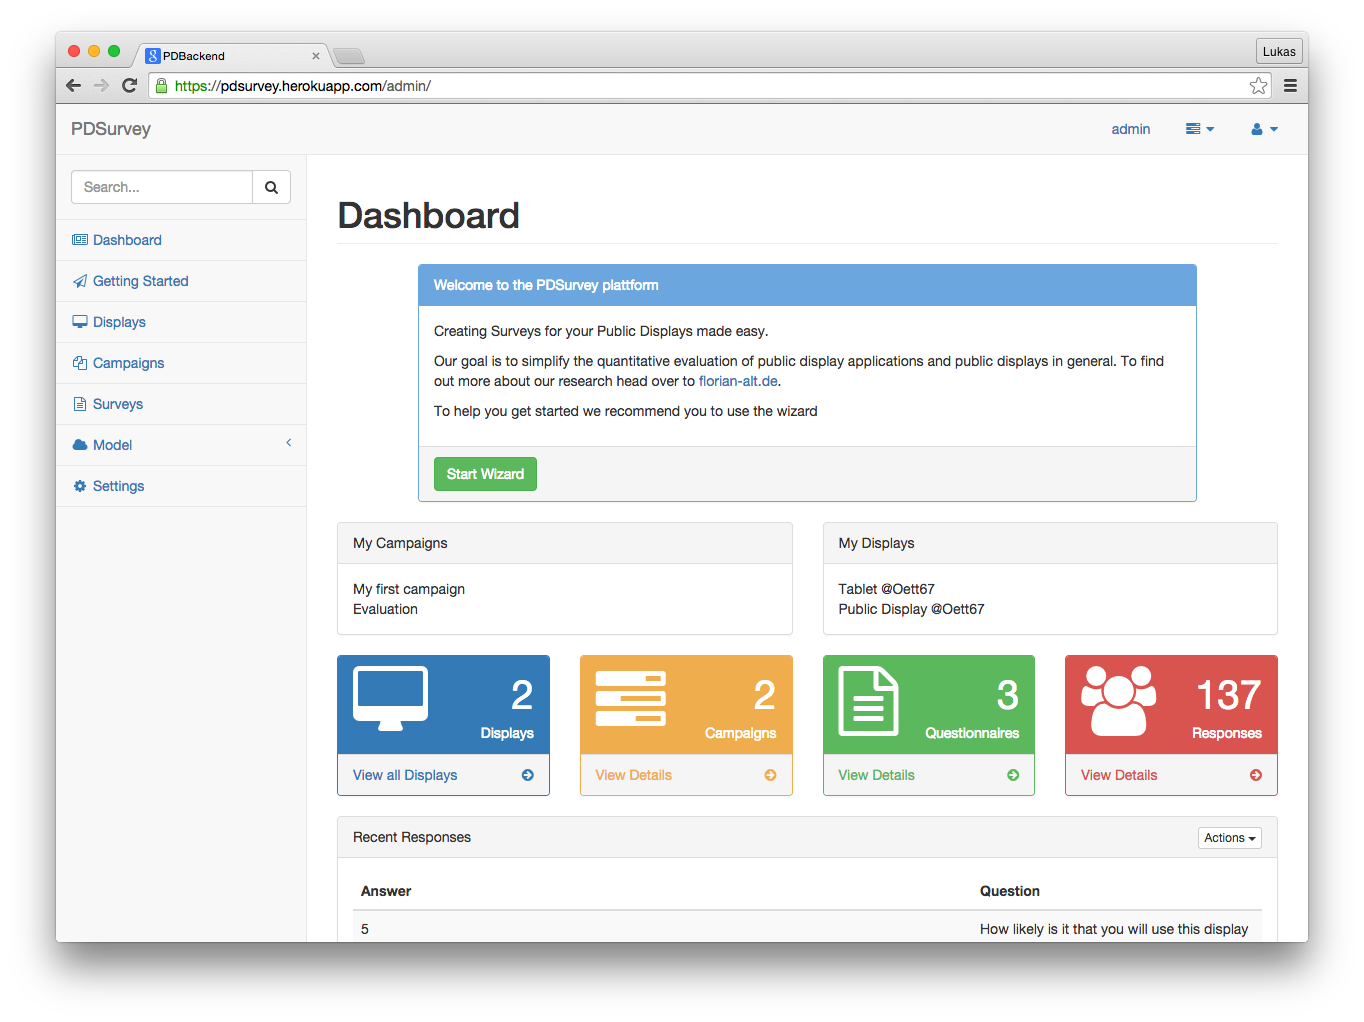
\includegraphics[width=\textwidth]{img/screenshots/pdadmin/dashboard}
		        \caption{Dashboard}
				\label{fig:pdadmin-dashobard}
		    \end{subfigure}
		    \hfill
		    \begin{subfigure}[b]{0.7\textwidth}
		        \centering
		        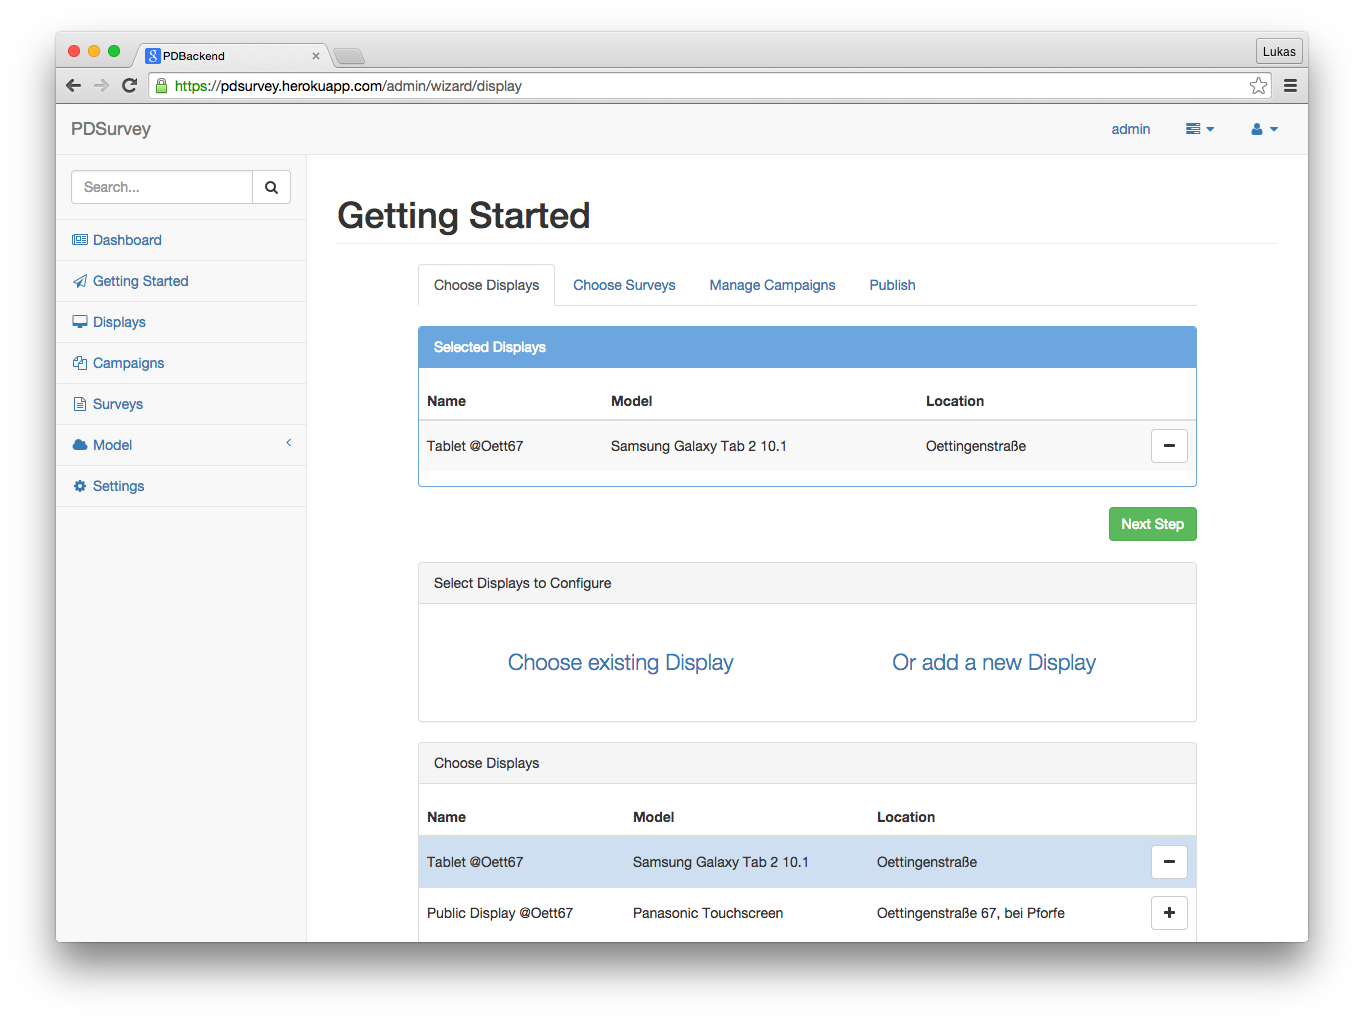
\includegraphics[width=\textwidth]{img/screenshots/pdadmin/wizard-display_selected.png}
		        \caption{Wizard}
		        \label{fig:pdadmin-wizard}
		    \end{subfigure}
		    \caption{Overview of PDAdmin.}
		\end{figure}
		


	\subsubsection{PDServer}

		The server was written in Node.js and to the outside only offers a RESTful API. All interactions users or developers make with the server are HTTP calls. When performing CRUD operations, all REST calls need to be executed and JSON objects are returned.
		Besides this REST functionality a rudimentary authentication mechanism is already implemented on the server and the capability for further logic, determining which client should ask which question next. This functionality might become of interest when trying to spread standardized questionnaires of longer length across multiple users or multiple displays. It would be intended for the server to keep track which questions have already been answered and to tell each instance of PDClient which question to ask next, in order to achieve a balanced question profile.
		The specification of PDServer's REST API can be found on GitHub\footnote{\url{https://github.com/lukasziegler/masterarbeit/tree/master/docs} (last accessed on April 15, 2015)} and on the enclosed CD (see Appendix \ref{appendix:cd-contents}).



	\subsubsection{PDClient}

		Our client tool was kept as simple and minimalistic as possible. The only communication between PDClient and PDAdmin is via REST calls, exchanging JSON objects. Even though both PDClient and PDAdmin are developed using Javascript frameworks, they have a separate code base. Reasons for this were on the one hand reduction of the application size, on the other hand different requirements of the client version and the administrator panel. PDClient needs to be highly scalable and offer a low latency and fast response time. For PDAdmin it is more important to offer a better usability and a more visual appealing presentation of the results. The goal is to reduce logic and complexity on client-side. Currently PDClient loads all questions for the questionnaire at startup and caches them for later access. 

		% Overview of elements
		PDClient has three main components (see figure \ref{fig:pdclient-screenshots}). The principal part is the \textit{Survey page}. All questions are loaded at once on startup. Then one question gets displayed at a time. Settings for the survey can be modified from PDBackend (e.g. number of questions to display and duration of the survey). Once the user makes a choice, it is directly logged on the server. In a case when a participant aborts answering the survey, the questions answered so far are still recorded. The \textit{About page} was added, since some employees from university said they were skeptical and had doubts regarding the research project, when there is no information whatsoever about which information is logged. To motivate people to participate, a \textit{Welcome page} was added. It turned out that a significantly larger number of people were willing to participate in a survey, after finding out that it will only take one minute, the research is university-related and that it will be used for a Master's thesis.


		\begin{figure}
		    \centering
		    \begin{subfigure}[b]{0.6\textwidth}
		        \centering
		        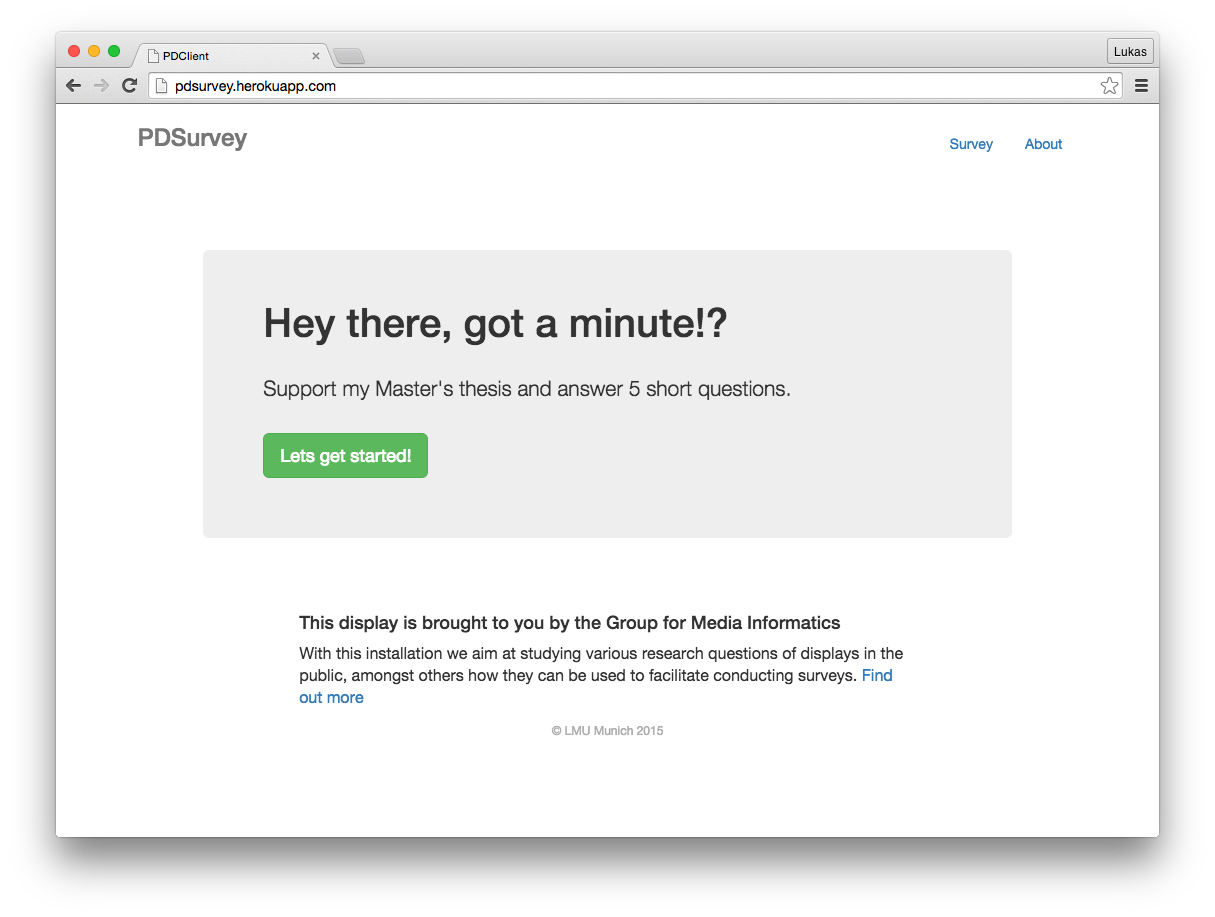
\includegraphics[width=\textwidth]{img/screenshots/pdclient/welcome}
		        \caption{Welcome Page}
		        \label{fig:4-pdclient-welcome}
		    \end{subfigure}
		    \hfill
		    \begin{subfigure}[b]{0.6\textwidth}
		        \centering
		        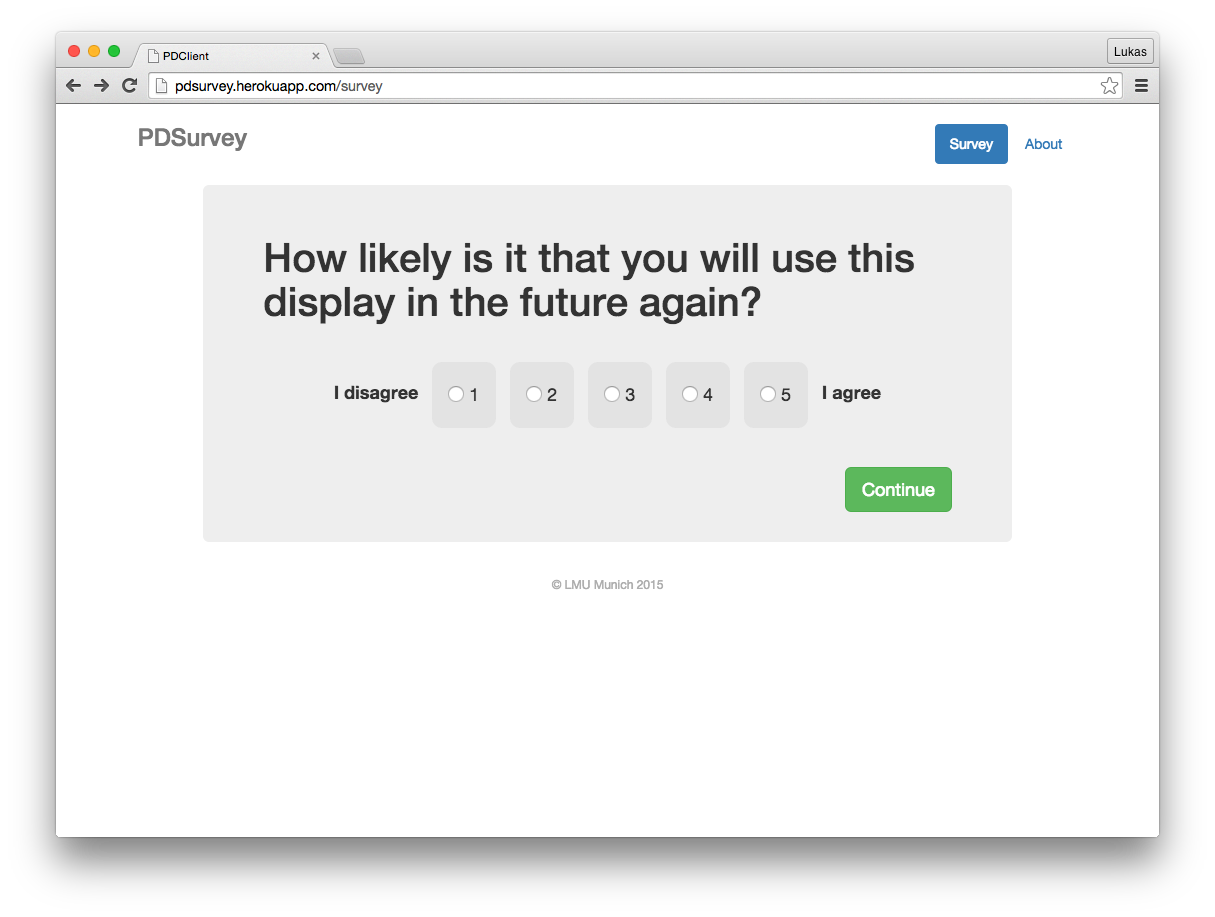
\includegraphics[width=\textwidth]{img/screenshots/pdclient/survey}
		        \caption{Survey page}
		        \label{fig:4-pdclient-survey}
		    \end{subfigure}
		    \hfill
		    \begin{subfigure}[b]{0.6\textwidth}
		        \centering
		        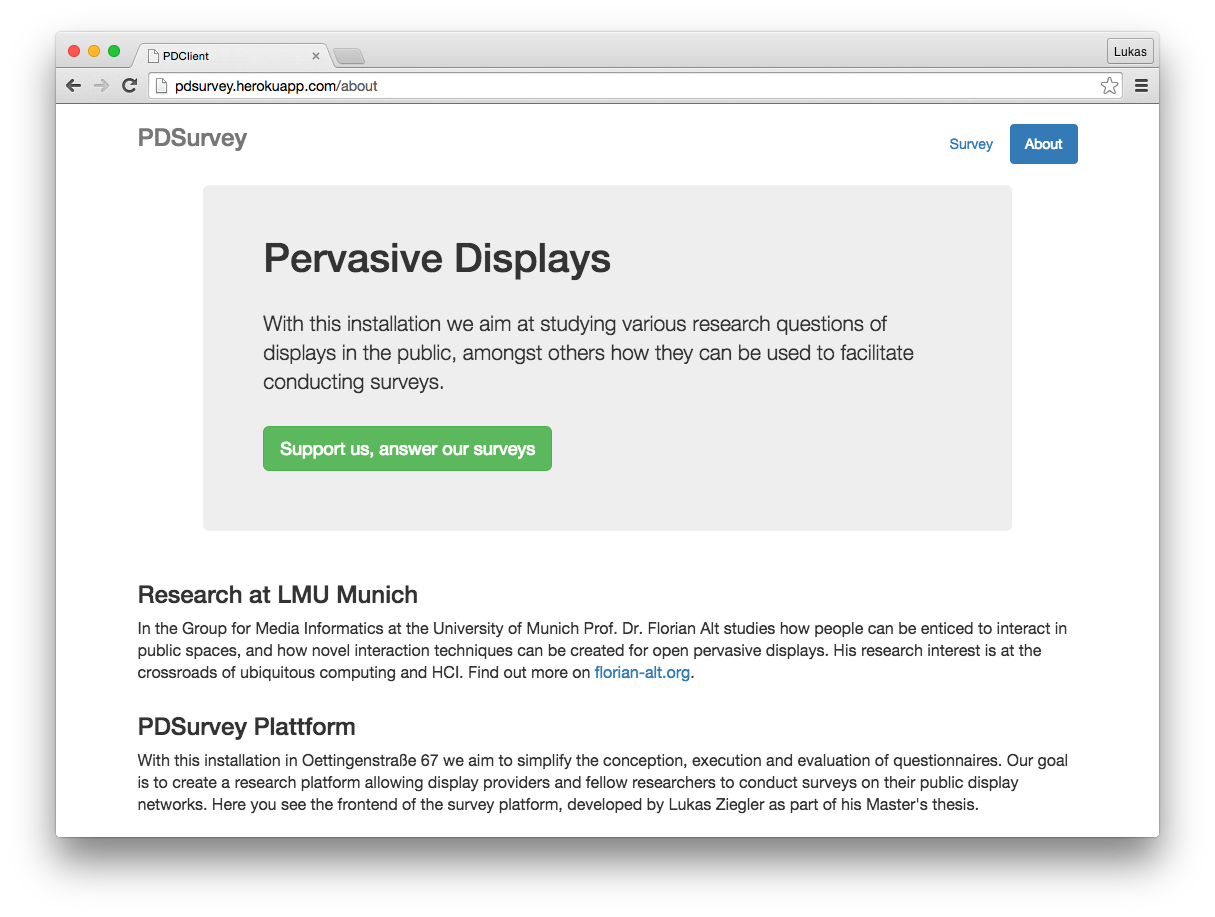
\includegraphics[width=\textwidth]{img/screenshots/pdclient/about}
		        \caption{About page}
		        \label{fig:4-pdclient-about}
		    \end{subfigure}
		    \caption{Overview of PDClient.}
		    \label{fig:pdclient-screenshots}
		\end{figure}



	\subsubsection{EmbedCode}

		Offering an embed code for surveys, turned out to be a pure proof-of-concept. The problem was that the Balloon Shooter game, on which \textit{PDSurvey} should be integrated, did not support any HTTP calls or overlays. Thus, we had to fall back on another solution. This embed code was intended to be used by display operators, wanting to include questionnaires hovering over their web-based public display applications (see figure \ref{fig:4-embed-code}). The technical realization was inspired by Web Bug \footnote{\url{http://en.wikipedia.org/wiki/Web_bug} (last accessed on November 26, 2014)}, and the embed code offered by Google Analytics\footnote{\url{https://developers.google.com/analytics/resources/concepts/gaConceptsTrackingOverview} (last accessed on November 26, 2014)}.

		% Implementation
		One minified line of JavaScript code needs to be added before the closing HTML <body>-tag. This minified line creates a <script>-tag in the Document Object Model (DOM) of the HTML page and injects a JavaScript file from the \textit{PDSurvey} platform. This personalized scripts first loads jQuery and/or Angular.js asynchronously, creates an instance of PDClient inside of the primary website's DOM. All questions for the questionnaire get loaded via PDServer's RESTful API and the responses get sent back to the server for logging. To avoid conflicts caused through the code injection, all classes and files are prefixed with a unique namespace. Depending on the type of implementation it is better to use jQuery or Angular.js \cite{AirPair2014jQueryAngular}. In the current prototype the full version of PDClient is not mirrored yet entirely to the browsers DOM.


	\begin{figure}
	    \begin{center}
	   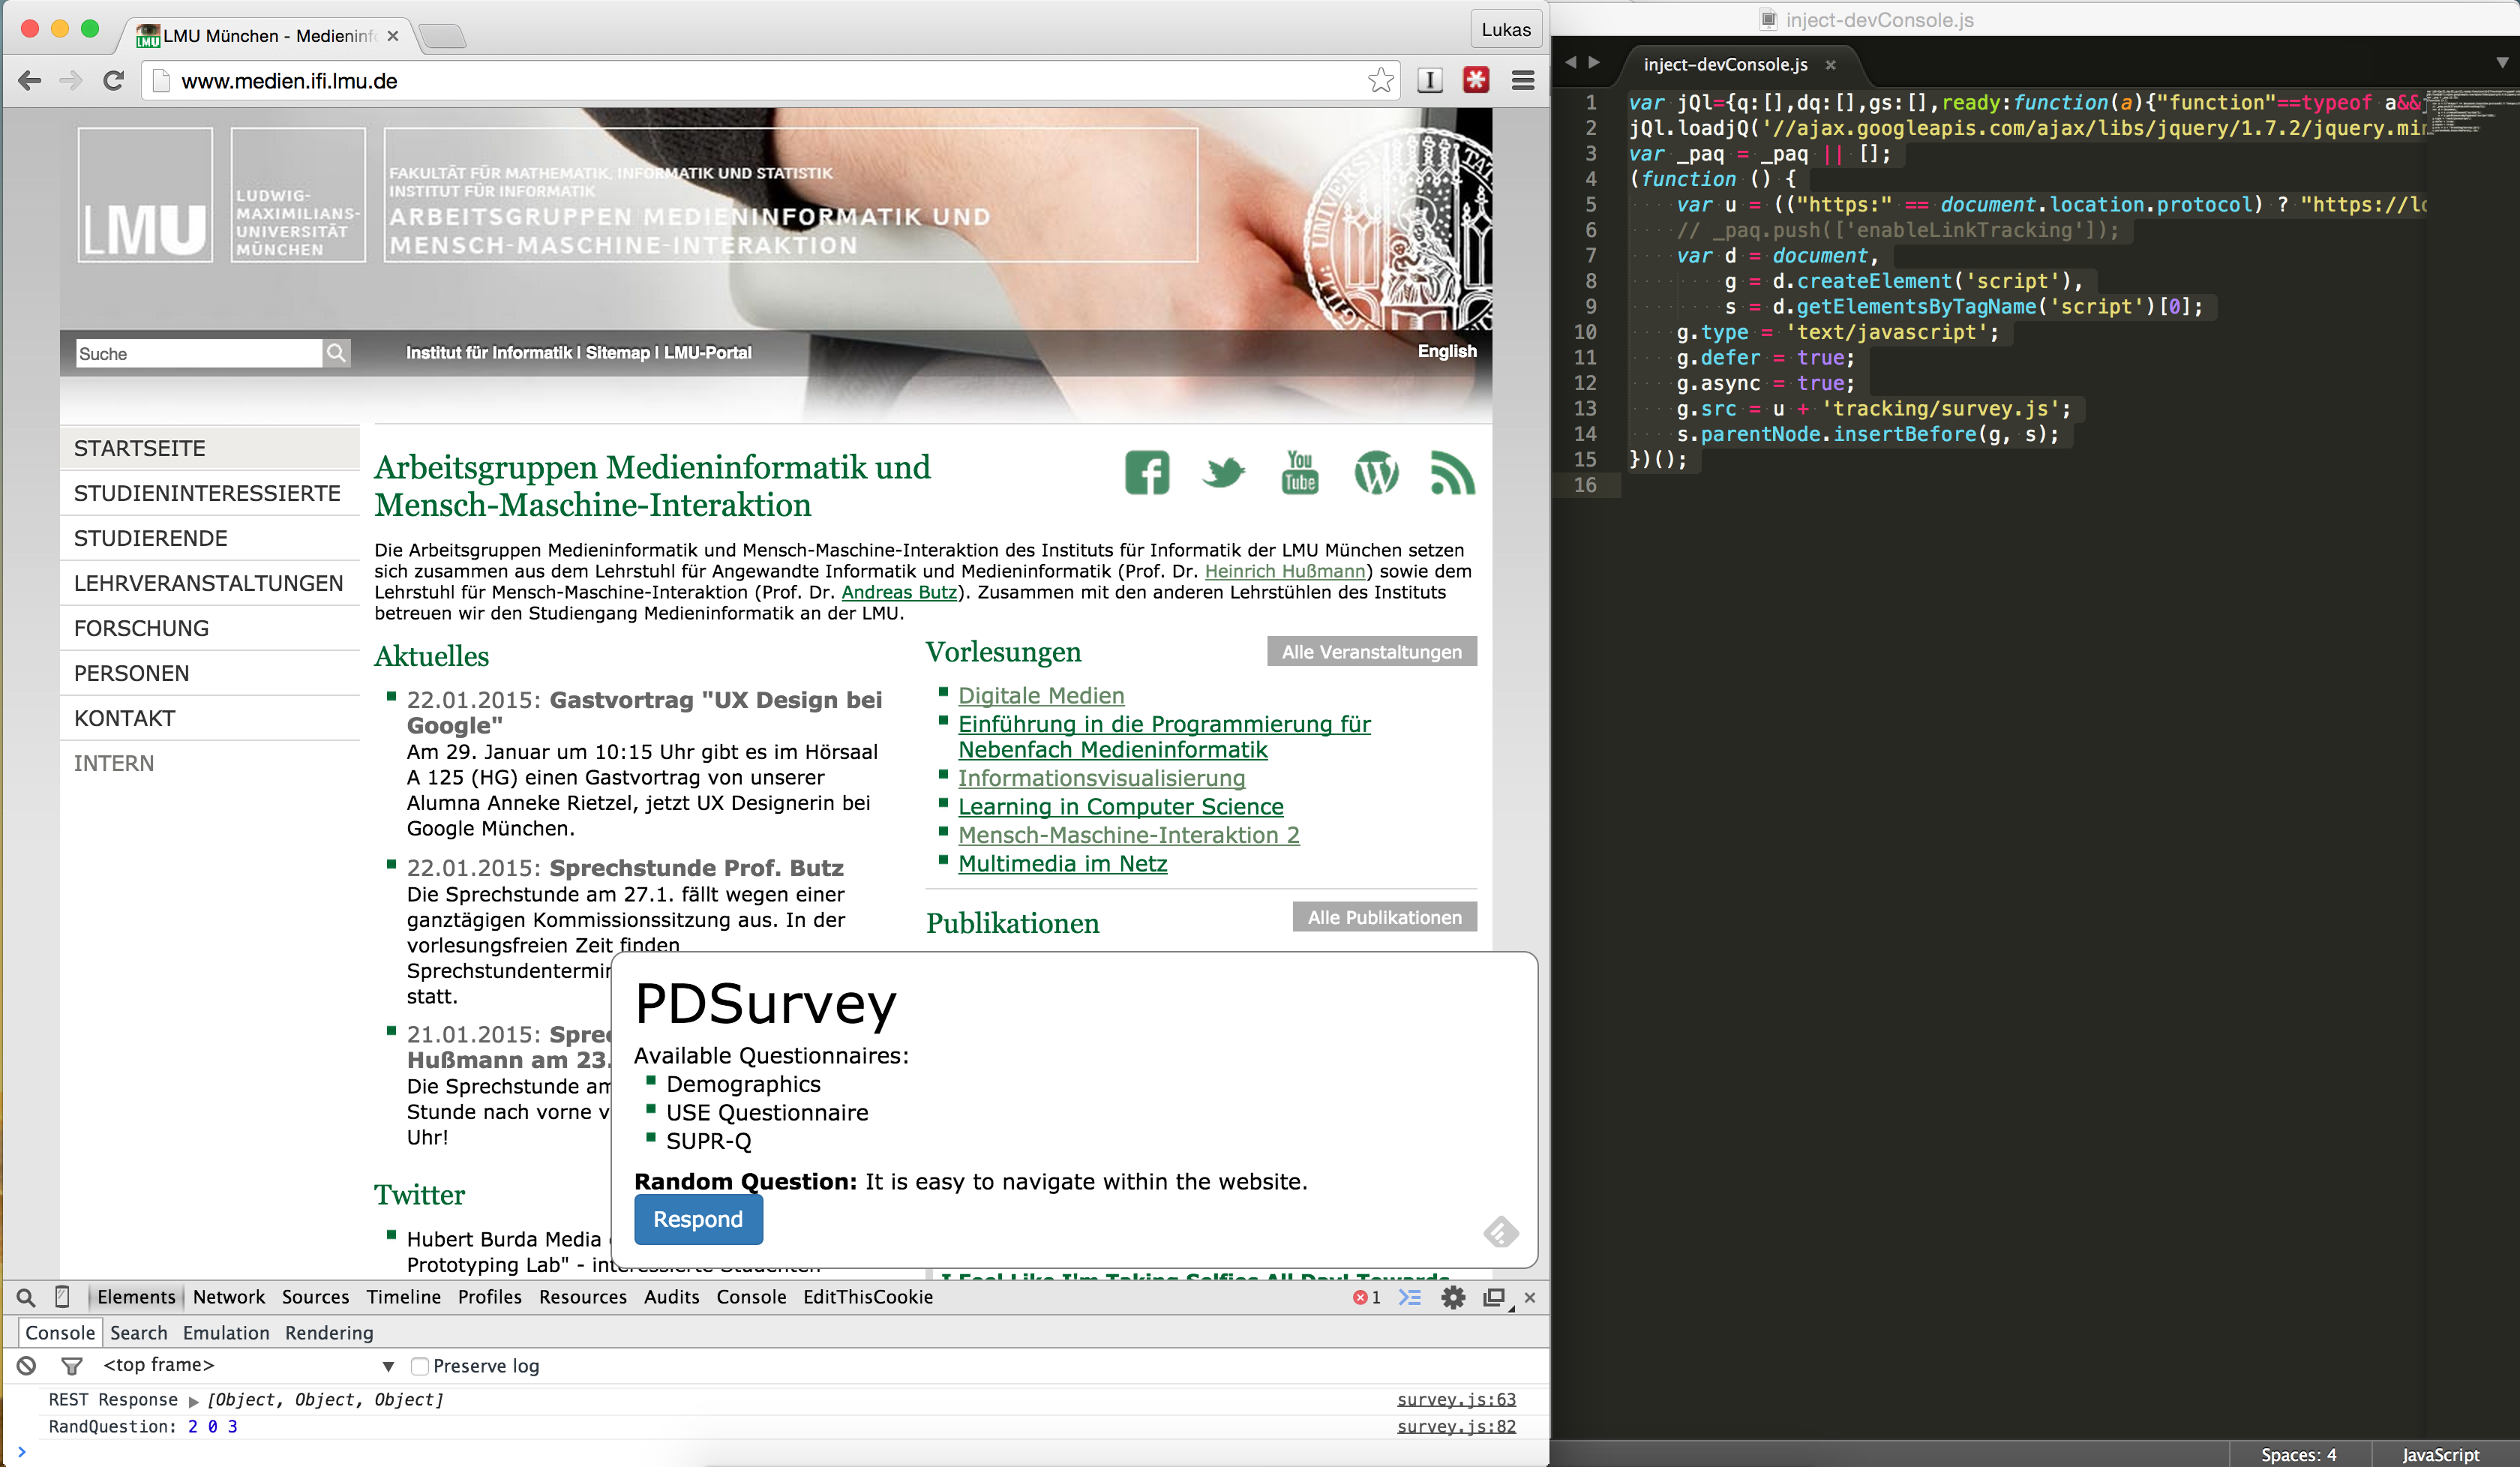
\includegraphics[width=.8\columnwidth]{img/screenshots/pdsurvey-overview/injection.png}
	    \end{center}
	 \caption[Embed Code]{Embed Code - Prototype for injecting a questionnaire on a remote website.}
	 \label{fig:4-embed-code}
	\end{figure}